\documentclass[12pt,prb,aps,epsf]{article}
\usepackage[utf8]{inputenc}
\usepackage{amsmath}
\usepackage{amsfonts}
\usepackage{amssymb}
\usepackage{graphicx} 
\usepackage{latexsym} 
\usepackage[toc,page]{appendix}
\usepackage{listings}
\usepackage{xcolor}
\usepackage{soul}
\usepackage[T1]{fontenc}
\usepackage{amsthm}
\usepackage{mathtools}
\usepackage{setspace}
\usepackage{array,multirow,makecell}
\usepackage{geometry}
\usepackage{textcomp}
\usepackage{float}
%\usepackage{siunitx}
\usepackage{cancel}
%\usepackage{tikz}
%\usetikzlibrary{calc, shapes, backgrounds, arrows, decorations.pathmorphing, positioning, fit, petri, tikzmark}
\usepackage{here}
\usepackage{titlesec}
%\usepackage{bm}
\usepackage{bbold}

\geometry{hmargin=2cm,vmargin=2cm}

\begin{document}
	
	\title{MP 34 Phénomènes de transports}
	\author{Laurent}
	
	\maketitle
	
	\tableofcontents
	
	\pagebreak
	
\section{Conduction électrique : loi d'Ohm locale}

\begin{eqnarray}
\vec{j} = \gamma \vec{E}
\end{eqnarray}
On a une tablette comprenant des fils (de cuivre) de différentes sections dont on va se servir pour expliciter la dépendance de la résistance en la section et la longueur.
On impose un courant $I$ sur un fil à l'aide d'un générateur de courant (on mesure I en mettant un ampèremètre en série) et on mesure la tension $U$ (au voltmètre) entre deux points séparés de la longueur L, puis on trace 
\begin{eqnarray}
R = \frac{U}{I} = \frac{L}{\gamma S}
\end{eqnarray}
en modélisant on montre ainsi que R dépend linéairement de L.\\
On peut ensuite, pour une longueur donnée, mesurer U avec différentes sections pour montrer que la résistance dépend de l'inverse de la section.\\
On peut ainsi finalement en déduire une estimation de la conductivité $\gamma$ pour le cuivre.

\section{Diffusion particulaire}

\begin{figure}[h]
\centerline{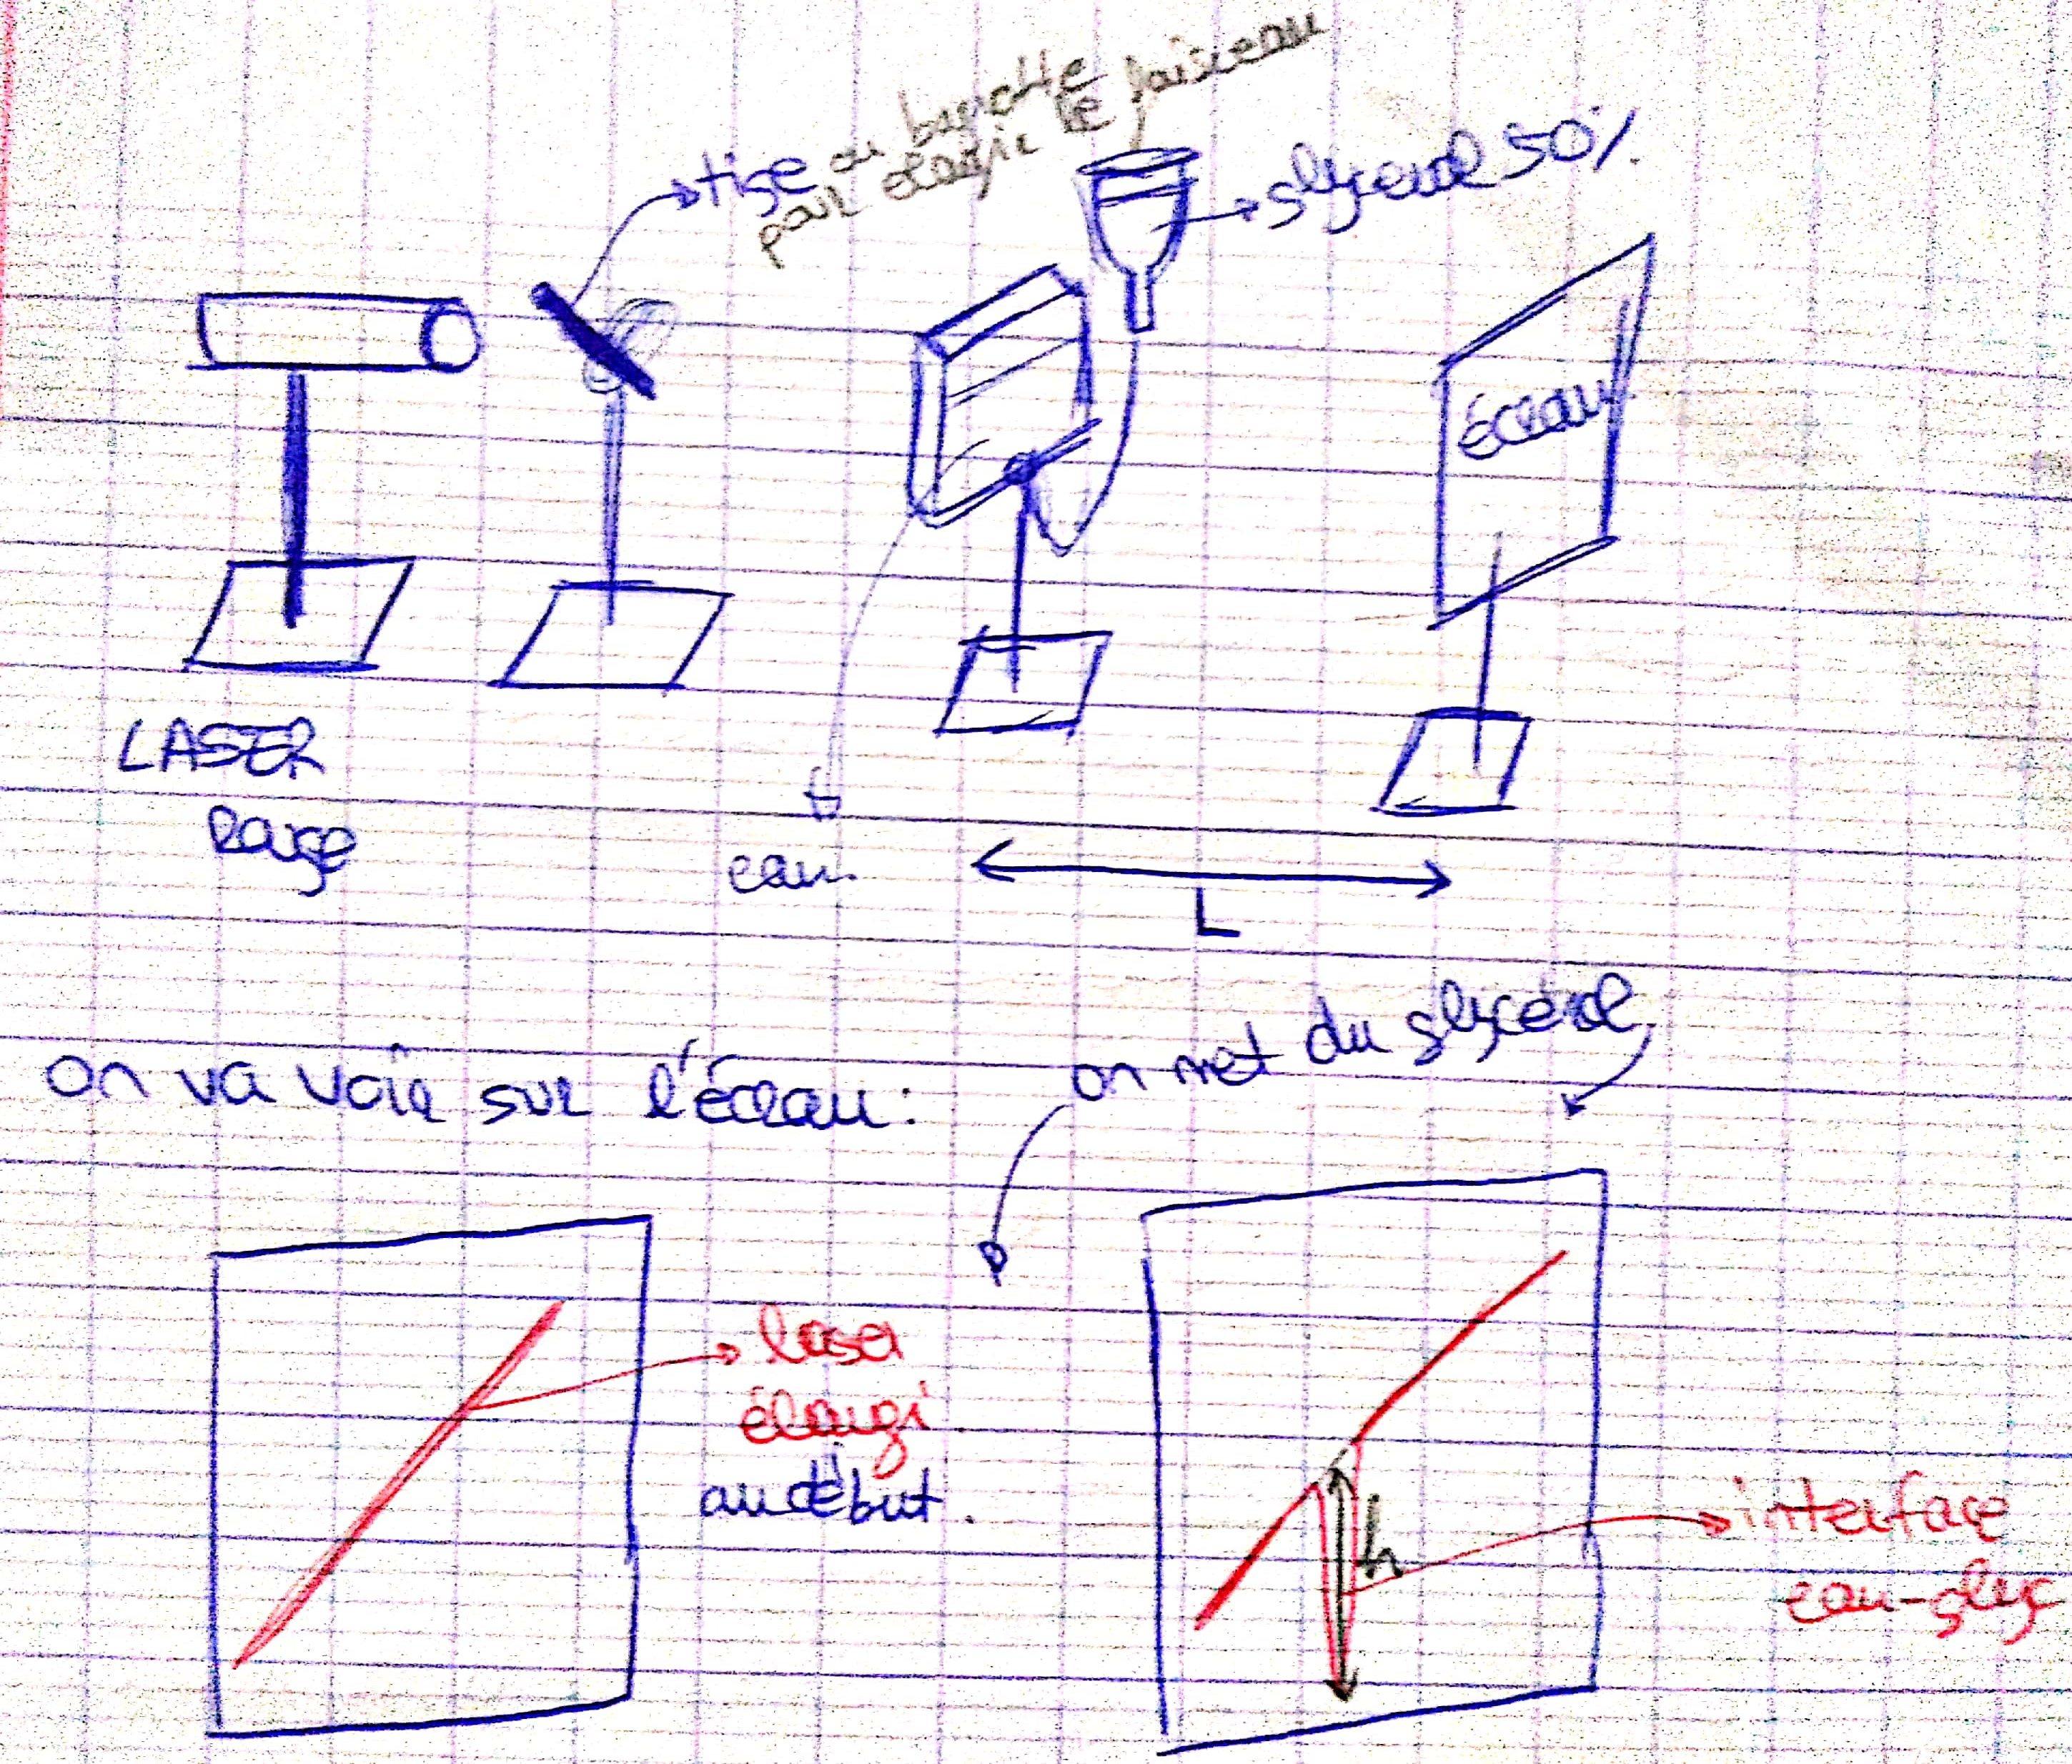
\includegraphics[width=13cm]{schema_diffusion}}
\end{figure}
On utilise une cuve avec une interface entre de l'eau et une solution de glycerol à 50\%. On envoie une nappe de lumière oblique sur la cuve à l'aide d'un laser et d'une baguette de verre. On regarde la figure obtenue par réfraction sur un écran derrière la cuve. On y voit une droite oblique, habillée d'un "pic" en son centre dû au gradient d'indice à l'interface : la hauteur $h$ de ce pic va alors nous permettre de remonter au coefficient de diffusion du glycerol.\\
En combinant équation de diffusion et optique on obtient 
\begin{eqnarray}
\alpha_{max} = \frac{(n_g-n_e)d}{4n_0\sqrt{\ln(2)Dt}}
\end{eqnarray}
avec $\alpha$ l'angle de déviation, L la distance entre l'écran et la cuve, $n_g$ l'indice optique du glycerol et $n_e$ celui de l'eau, $D$ le coefficient de diffusion, et $d$ l'épaisseur de la cuve. On en déduit 
\begin{eqnarray}
\tan \alpha = \frac{h}{L}\;\;\Rightarrow\;\; \frac{1}{\arctan^2{\frac{h}{l}}} = \frac{16n_0^2\ln2\,D}{d(n_g-n_e)}t
\end{eqnarray}
On va donc mesurer $h$ et tracer $\frac{1}{\arctan^2{\frac{h}{l}}}$ en fonction du temps, modéliser par une droite. A partir du coefficient directeur de cette droite $a$ on peut alors déduire la valeur du coefficient de diffusion
\begin{eqnarray}
D = \frac{ad(n_g-n_e)}{16n_0^2\ln2}\hspace{1cm} \frac{u(D)}{D} \simeq \frac{u(a)}{a}
\end{eqnarray}
On pourra ensuite vérifier que $D$ est bien dans l'intervalle attendu 
\begin{eqnarray}
D_{att} \in [1,10].10^{-10}\,\mathrm{m}^3.s^{-1}
\end{eqnarray}

\section{Diffusion de quantité de mouvement}
On fait ici une mesure de la viscosité à l'aide d'un vase de Mariotte, on pourra donc se référer au MP 03 Dynamique des fluides.

\section*{Questions}
\begin{itemize}
\item Quelle est l'unité de la viscosité ?\\
$\eta$ est en Pa.s

\item Comment définireriez vous la viscosité ?

\item Manip surprise : montrer que la résistance est inversement proportionnelle à la section.

\item Pourquoi les phénomènes de transports sont ils irréversibles ?

\item énoncé du second principe de la thermodynamique ?

\item Y a t'il un rapport entre ces phénomènes de transport et l'entropie ?

\section*{Remarques}
Pour introduire la viscosité on écrit Navier Stokes : dans le cas où le terme convectif est nul et où il n'y a pas de force volumique on obtient une équation de diffusion avec pour coefficient de diffusion $\eta/\rho$.

\end{itemize}

	
\end{document}